

\typeout{IJCAI--PRICAI--20 Instructions for Authors}



\documentclass{article}
\pdfpagewidth=8.5in
\pdfpageheight=11in
\usepackage{ijcai20}

\usepackage{times}
\usepackage{soul}
\usepackage{url}
\usepackage[hidelinks]{hyperref}
\usepackage[utf8]{inputenc}
\usepackage[small]{caption}
\usepackage{graphicx}
\usepackage{amsmath}
\usepackage{amssymb}
\usepackage{amsthm}
\usepackage{booktabs}
\usepackage{algorithm}
\usepackage{algorithmic}
\usepackage{multirow}
\usepackage{color}
\usepackage{array}

\usepackage{pgfplots}
\usepackage{tikz}
\usepackage{subfigure}
\usepackage{latexsym}
\usepackage{tikz-qtree}
\usepackage{hyperref}
\usepgflibrary{arrows.meta}
\usetikzlibrary{fit, calc, decorations.pathreplacing, positioning, shapes.geometric}

\urlstyle{same}

\newcommand{\specialcell}[2][c]{\begin{tabular}[#1]{@{}c@{}}#2\end{tabular}}



\newtheorem{example}{Example}
\newtheorem{theorem}{Theorem}







\title{Fast and Accurate Neural CRF Constituency Parsing}





\author{
Yu Zhang\thanks{Yu Zhang and Houquan Zhou make equal contributions to this work. Zhenghua Li is the corresponding author.},
Houquan Zhou$^{\ast}$,
Zhenghua Li
\affiliations
Institute of Artificial Intelligence, School of Computer Science and Technology, \\ Soochow University, Suzhou, China \\
\emails
yzhang.cs@outlook.com,
hqzhou@stu.suda.edu.cn,
zhli13@suda.edu.cn
}


\begin{document}
\maketitle

\begin{abstract}
\label{section:abstract}

Estimating probability distribution is one of the core issues in the NLP field. However, in both deep learning (DL) and pre-DL eras, unlike the vast applications of linear-chain CRF in sequence labeling tasks, very few works have applied tree-structure CRF to constituency parsing, mainly due to the complexity and inefficiency of the inside-outside algorithm.
This work presents a fast and accurate neural CRF constituency parser. The key idea is to batchify the inside algorithm for loss computation by direct large tensor operations on GPU, and meanwhile avoid the outside algorithm for gradient computation via efficient back-propagation.
We also propose a simple two-stage bracketing-then-labeling parsing approach to improve efficiency further.
To improve the parsing performance, inspired by recent progress in dependency parsing, we introduce a new scoring architecture
based on boundary representation and biaffine attention, and a beneficial dropout strategy.
Experiments on PTB, CTB5.1, and CTB7 show that our two-stage CRF parser achieves new state-of-the-art performance on both settings of w/o and w/ BERT, and can parse over 1,000 sentences per second.
We release our code at https://github.com/yzhangcs/crfpar.

\end{abstract} \section{Introduction}
\label{section:introduction}

Given an input sentence, constituency parsing aims to build a hierarchical tree as depicted in Figure~\ref{fig:const-tree-original}, where the leaf or terminal nodes correspond to input words and non-terminal nodes are constituents (e.g., $\texttt{VP}_{3,5}$).
As a fundamental yet challenging task in the natural language processing (NLP) field, constituency parsing has attracted a lot of research attention since large-scale treebanks were annotated,  such as Penn Treebank (PTB), Penn Chinese Treebank (CTB), etc.
Parsing outputs are also proven to be extensively useful for a wide range of downstream applications \cite{akoury-etal-2019-syntactically,wang-etal-2018-tree}.


As one of the most influential works, \citeauthor{collins-1997-three}~\shortcite{collins-1997-three} extends methods from probabilistic context-free grammars (PCFGs) to lexicalized grammars.
Since then, constituency parsing has been dominated by such generative models for a long time, among which
the widely used Berkeley parser adopts an unlexicalized PCFG with latent non-terminal splitting annotations \cite{matsuzaki-etal-2005-probabilistic,petrov-klein-2007-improved}.
As for discriminative models, there exist two representative lines of research.
The first line adopts the graph-based view based on dynamic programming decoding, using either local max-entropy estimation \cite{kaplan-etal-2004-speed} or global max-margin training \cite{taskar-etal-2004-max}.
The second group builds a tree via a sequence of shift-reduce actions based on greedy or beam decoding, known as the transition-based view \cite{sagae-lavie-2005-classifier,zhu-etal-2013-fast}.








\begin{figure}[tb]
\subfigure[original tree]
{
\label{fig:const-tree-original}
  \begin{minipage}[b]{0.22\textwidth}
      \centering
      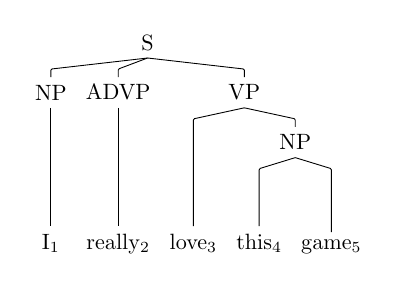
\begin{tikzpicture}[
          scale=0.8,
          level distance=22.5pt,
          every tree node/.style={align=center,anchor=base},
          frontier/.style={distance from root=90pt},
          edge from parent/.style={draw,edge from parent path={(\tikzparentnode.south) {[rounded corners=0.5pt]-- ($(\tikzchildnode |- \tikzparentnode.south) + (0, -5pt)$) -- (\tikzchildnode)}}}
          ]
      \Tree
      [.S
          [.NP I$_1$ ]
          [.ADVP really$_2$ ]
          [.VP love$_3$ [.NP this$_4$ game$_5$ ] ] ];
  \end{tikzpicture}

  \end{minipage}
}
\hfill
\subfigure[CNF tree (left binarized)]
{
\label{fig:binaried-tree}
  \begin{minipage}[b]{0.22\textwidth}
      \centering
      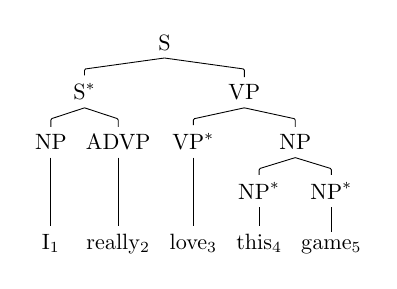
\begin{tikzpicture}[
          scale=0.8,
          level distance=22.5pt,
          every tree node/.style={align=center,anchor=base},
          frontier/.style={distance from root=90pt},
          edge from parent/.style={draw,edge from parent path={(\tikzparentnode.south) {[rounded corners=0.5pt]-- ($(\tikzchildnode |- \tikzparentnode.south) + (0, -5pt)$) -- (\tikzchildnode)}}}
        ]
      \Tree
          [.S
          [.$\textrm{S}^\ast$ [.NP I$_1$ ] [.ADVP really$_2$ ] ]
          [.VP
            [.$\textrm{VP}^\ast$ love$_3$ ]
            [.NP [.$\textrm{NP}^\ast$ this$_4$ ]
                 [.$\textrm{NP}^\ast$ game$_5$ ] ] ] ];
      \end{tikzpicture}
  \end{minipage}
}
\caption{
    Example constituency trees. Part-of-speech (POS) tags are not used  as inputs in this work and thus excluded.
}
\label{fig:const-tree-full-figure}
\end{figure}
 
Recently, constituency parsing has achieved significant progress thanks to the impressive capability of deep neural networks in context representation.
Two typical and popular works are respectively the transition-based parser of \citeauthor{cross-huang-2016-span}~\shortcite{cross-huang-2016-span} and the graph-based parser of \citeauthor{stern-etal-2017-minimal}~\shortcite{stern-etal-2017-minimal}.
As discriminative models, the two parsers share several commonalities, both using 1) multi-layer BiLSTM as encoder; 2) minus features from BiLSTM outputs as span representations; 3) MLP for span scoring; 4) max-margin training loss.
Most works \cite{gaddy-etal-2018-whats,kitaev-klein-2018-constituency} mainly follow the two parsers and achieve much higher parsing accuracy than traditional non-neural models, especially with contextualized word representations trained with language modeling loss on large-scale unlabeled data \cite{peters-etal-2018-deep,devlin-etal-2019-bert}.

Despite the rapid progress, existing constituency parsing research suffers from two closely related drawbacks. First, parsing (also for training) speed is slow and can hardly satisfy the requirement of real-life systems.
Second, the lack of explicitly modeling tree/subtree probabilities may hinder the effectiveness of utilizing parsing outputs.
On the one hand, estimating probability distribution is one of the core issues in the NLP field \cite{le-zuidema-2014-inside}. On the other hand, compared with unbounded tree scores, tree probabilities can better serve high-level tasks as soft features \cite{jin-etal-2020-relation},
and marginal probabilities of subtrees can support
the more sophisticated Minimum Bayes Risk (MBR) decoding \cite{smith-smith-2007-probabilistic}.

In fact, \citeauthor{finkel-etal-2008-efficient}~\shortcite{finkel-etal-2008-efficient} and \citeauthor{durrett-klein-2015-neural}~\shortcite{durrett-klein-2015-neural} both propose CRF-based constituency parsing by directly modeling the conditional probability. However, both models are extremely inefficient due to
the high time-complexity of the inside-outside algorithm for loss and gradient computation, especially the outside procedure.
The issue becomes more severe in the DL era since all previous works perform the inside-outside computation on CPUs according to our knowledge and switching between GPU and CPU is expensive.




This work proposes a fast and accurate CRF constituency parser by substantially extending the graph-based parser of \citeauthor{stern-etal-2017-minimal}~\shortcite{stern-etal-2017-minimal}. The key contribution is that we batchify the inside algorithm for direct loss and gradient computation on GPU. Meanwhile, we find that the outside algorithm can be efficiently fulfilled by automatic back-propagation, which is shown to be equally efficient with the inside (forward) procedure, naturally verifying the great theoretical work of \citeauthor{eisner-2016-inside}~\shortcite{eisner-2016-inside}.
Similarly, we batchify the Cocke–Kasami–Younger (CKY) algorithm for fast decoding.

In summary, we make the following contributions.
\begin{itemize}
\item We for the first time propose a fast and accurate CRF constituency parser for directly modeling (marginal) probabilities of trees and subtrees.
The efficiency issue, which bothers the community for a long time, is well solved by elegantly batchifying the inside and CKY algorithms for direct computation on GPU.




\item We propose a two-stage bracketing-then-labeling parsing approach that is more efficient and achieves slightly better performance than the one-stage method.



\item We propose a new span scoring architecture based on span boundary representation and biaffine attention scoring, which performs better than the widely used minus-feature method. We also show that the parsing performance can be improved by a large margin via better parameter settings such as dropout configuration.

\item Experiments on three English and Chinese benchmark datasets show that our proposed two-stage CRF parser achieves new state-of-the-art parsing performance under both settings of w/o and w/ BERT \cite{devlin-etal-2019-bert}).
In terms of parsing speed, our parser can parse over 1,000 sentences per second.



\end{itemize}


\begin{figure}[tb]
\centering
\includegraphics [scale=0.8] {figures/framework.pdf}
\caption{Model architecture.
}
\label{fig:framework}
\end{figure}










%
 \section{Two-stage CRF Parsing}
\label{section:2stage-parsing}

Formally, given a sentence consisting of $n$ words  $\boldsymbol{x}=w_0,\dots, w_{n-1}$,
a constituency parse tree, as depicted in Figure~\ref{fig:const-tree-original}, is denoted as $\boldsymbol{t}$, and $(i,j,l) \in \boldsymbol{t}$ is a constituent spanning $w_{i}...w_{j}$ with a syntactic label $l \in \mathcal{L}$.
Alternatively, a tree can be factored into two parts, i.e., $\boldsymbol{t}=(\boldsymbol{y}, \boldsymbol{l})$, where $\boldsymbol{y}$ is an unlabeled (a.k.a. bracketed) tree and $\boldsymbol{l}$ is a label sequence for all constituents in a certain order.
Interchangeably, $(3,5, \texttt{VP})$ is also denoted as $\texttt{VP}_{3,5}$.




To accommodate the inside and CKY algorithms, we transform the original tree into
those of Chomsky normal form (CNF) using the NLTK tool\footnote{\url{https://www.nltk.org}}, as shown in Figure~\ref{fig:binaried-tree}.
Particularly, consecutive unary productions such as $\texttt{X}_{i,j} \rightarrow \texttt{Y}_{i,j}$ are collapsed into one $\texttt{X+Y}_{i,j}$.
We adopt left binarization since preliminary experiments show it is slightly superior to right binarization.
After obtaining the 1-best tree via CKY decoding, the CNF tree is recovered into the \textit{n}-ary form.




\subsection{Model Definition} \label{sec:model-defination}
\label{sub@section:model-definition}

In this work, we adopt a two-stage bracketing-then-labeling framework for constituency parsing, which we show not only simplifies the model architecture but also improves efficiency, compared with the traditional one-stage approach adopted in previous works \cite{stern-etal-2017-minimal,gaddy-etal-2018-whats}.





\paragraph{First stage: bracketing.}
Given $\boldsymbol{x}$, the goal of the first stage is to find an optimal unlabeled tree $\boldsymbol{y}$.
The score of a tree is decomposed into the scores of all contained constituents.
\begin{equation} \label{equation:tree-score}
s(\boldsymbol{x},\boldsymbol{y}) = \sum\limits_{(i,j)\in \boldsymbol{y}}s(i,j)
\end{equation}
Under CRF, the conditional probability is
\begin{equation}\label{equation:tree-prob}
\begin{split}
& p(\boldsymbol{y}\mid\boldsymbol{x})  = \frac{e^{s(\boldsymbol{x},\boldsymbol{y})}}{Z(\boldsymbol{x}) \equiv \sum\limits_{\boldsymbol{y'} \in \mathcal{T}(\boldsymbol{x})} {e^{s(\boldsymbol{x},\boldsymbol{y'})}}}
\end{split}
\end{equation}
where $Z(\boldsymbol{x})$ is known as the normalization term, and $\mathcal{T}(\boldsymbol{x})$ is the set of legal trees.

Given all constituent scores $s(i,j)$, we use the CKY algorithm to find the optimal tree $\hat{\boldsymbol{y}}$.
\begin{equation} \label{equation:tree-argmax}
\hat{\boldsymbol{y}} = \arg\max_{\boldsymbol{y}} s(\boldsymbol{x}, \boldsymbol{y}) = \arg\max_{\boldsymbol{y}} p(\boldsymbol{y} \mid \boldsymbol{x})
\end{equation}






\paragraph{Second stage: labeling.}
Given a sentence $\boldsymbol{x}$ and a tree $\boldsymbol{y}$, the second stage independently predicts a label for each constituent $(i,j) \in \boldsymbol{y}$.
\begin{equation} \label{equation:label-argmax}
\hat{l} = \arg\max_{l \in \mathcal{L}} s(i,j,l)
\end{equation}
Note that we use gold-standard unlabeled trees for loss computation during training.
For a sentence of length $n$, all CNF trees contain the same $2n-1$ constituents. Therefore, this stage has a time complexity of $O(n|\mathcal{L}|)$.



\paragraph{Time complexity analysis.}
The CKY algorithm has a time complexity of $O(n^3)$. Therefore, the time complexity of our two-stage parsing approach is $O(n^3+n|\mathcal{L}|)$.
In contrast, for the one-stage parsing approach, the CKY algorithm needs to determine the best label for all $n^2$ spans and thus needs
$O(n^3+n^2|\mathcal{L}|)$, where $|\mathcal{L}|$ is usually very large (e.g., 138 for English in Table~\ref{table:statistics}).





\subsection{Scoring Architecture}

This subsection introduces the network architecture for scoring spans and labels, as shown in Figure~\ref{fig:framework}, which
mostly follows \citeauthor{stern-etal-2017-minimal}~\shortcite{stern-etal-2017-minimal} with two important modifications: 1) boundary representation and biaffine attention for score computation; 2) better parameter settings following \citeauthor{Timothy-d17-biaffine}~\shortcite{Timothy-d17-biaffine}.


\paragraph{Inputs.}
For the $i$th word, its input vector $\mathbf{e}_i$ is the concatenation of the word embedding and character-level representation:
\begin{equation} \label{equation:token-representation}
\mathbf{e}_i = \mathbf{e}^{word}_i \oplus \mathrm{CharLSTM}(w_i)
\end{equation}
where
$\mathrm{CharLSTM}(w_i)$ is the output vectors after feeding the character sequence into a BiLSTM layer \cite{lample-etal-2016-neural}.
Previous works show that replacing POS tag embeddings with $\mathrm{CharLSTM}(w_i)$ leads to consistent improvement \cite{kitaev-klein-2018-constituency}.
This can also simplify the model without the need of predicting POS tags (n-fold jack-knifing on training data).


\paragraph{BiLSTM encoder.}
We employ three BiLSTM layers over the input vectors for context encoding.
We denote as $\mathbf{f}_i$ and $\mathbf{b}_i$ respectively the output vectors of the top-layer forward and backward LSTMs for $w_i$.



In this work, we borrow most parameter settings from the dependency parser of \citeauthor{Timothy-d17-biaffine}~\shortcite{Timothy-d17-biaffine}. We find that the dropout strategy is very crucial for parsing performance,
which differs from the vanilla implementation of \citeauthor{stern-etal-2017-minimal}~\shortcite{stern-etal-2017-minimal} in two aspects.

First, for each word $w_i$, $\mathbf{e}^{word}_i$ and $\mathrm{CharLSTM}(w_i)$ are dropped as a whole, either unchanged or becoming a $\mathbf{0}$ vector.
If one vector is dropped into $\mathbf{0}$, the other is compensated with a ratio of 2.
Second, the same LSTM layer shares the same dropout masks at different timesteps (words).





\paragraph{Boundary representation.}

For each word $w_i$, we compose the context-aware word representation following \citeauthor{stern-etal-2017-minimal}~\shortcite{stern-etal-2017-minimal}.\footnote{Our preliminary experiments show that $\mathbf{f}_i \oplus \mathbf{b}_{i+1}$ achieves consistent improvement over $\mathbf{f}_i \oplus \mathbf{b}_i$. The possible reason may be that both $\mathbf{f}_i$ and $\mathbf{b}_i$ use $\mathbf{e}_i$ as input and thus provide redundant information.}
\begin{equation}
\mathbf{h}_i = \mathbf{f}_i \oplus \mathbf{b}_{i+1}
\end{equation}
The dimensions of $\mathbf{h}_i$ is 800.

Instead of directly applying a single MLP to $\mathbf{h}_i$,
we observe that a word must act as either left or right boundaries in all constituents in a given tree.
Therefore, we employ two MLPs to make such distinction and obtain left and right boundary representation vectors.
\begin{equation}
\label{mlp-borlders}
\mathbf{r}_i^{l}; \mathbf{r}_i^{r} =\mathrm{MLP}^{l} \left( \mathbf{h}_i \right); \mathrm{MLP}^{r} \left( \mathbf{h}_i \right)
\end{equation}
The dimension $d$ of $\mathbf{r}_i^{l/r}$ is 500.
As pointed out by \citeauthor{Timothy-d17-biaffine}~\shortcite{Timothy-d17-biaffine}, MLPs reduce the dimension of $\mathbf{h}_i$ and, more importantly, detain only syntax-related information, thus alleviating the risk of over-fitting.


\paragraph{Biaffine scoring.}

Given the boundary representations,
we score each candidate constituent $(i,j)$ using biaffine operation
over the left boundary representation of $w_i$ and the right boundary representation of $w_j$.
\begin{equation} \label{equation:biaffine}
s(i,j) =  \left[
\begin{array}{c}
  \mathbf{r}_{i}^{l} \\
    1
\end{array}
\right]^\mathrm{T}
\mathbf{W} \mathbf{r}_{j}^{r}
\end{equation}
where $\mathbf{W} \in \mathbb{R}^{d \times d}$.


It is analogous to compute scores of constituent labels $s(i,j,l)$.
Two extra MLPs are applied to $\mathbf{h}_i$ to obtain boundary representations $\bar{\mathbf{r}}^{l/r}_i$ (with dimension $\bar{d}$).
We then use $|\mathcal{L}|$ biaffines ($\mathbb{R}^{\bar{d} \times \bar{d}}$) to obtain all label scores.
Since $|\mathcal{L}|$ is large, we use a small dimension $\bar{d}$ of 100 for $\bar{\mathbf{r}}^{l/r}_i$ (vs. 500 for ${\mathbf{r}}^{l/r}_i$) to reduce memory and computation cost.

\paragraph{Previous scoring method.}
\citeauthor{stern-etal-2017-minimal}~\shortcite{stern-etal-2017-minimal} use minus features of BiLSTM outputs as span representations \cite{wang-chang-2016-graph,cross-huang-2016-span} and apply MLPs to compute span scores.
\begin{equation} \label{equation:minus-score}
s(i,j)=\mathrm{MLP}(\mathbf{h}_{i}-\mathbf{h}_{j})
\end{equation}
We show that our new scoring method is clearly superior in the experiments.


\subsection{Training Loss}

For a training instance $(\boldsymbol{x}, \boldsymbol{y}, \boldsymbol{l})$, The training loss is composed of two parts.
\begin{equation} \label{equation:final-loss}
\mathit{L(\boldsymbol{x}, \boldsymbol{y}, \boldsymbol{l})} = \mathit{L}^{bracket}(\boldsymbol{x}, \boldsymbol{y}) + \mathit{L}^{label}(\boldsymbol{x}, \boldsymbol{y}, \boldsymbol{l})
\end{equation}
The first term is the sentence-level global CRF loss, trying to maximize the conditional probability:
\begin{equation}\label{equation:bracket-loss}
\begin{split}
\mathit{L}^{bracket}(\boldsymbol{x},\boldsymbol{y})
&= -s(\boldsymbol{x}, \boldsymbol{y}) + \log Z(\boldsymbol{x})
\end{split}
\end{equation}
where $\log Z(\boldsymbol{x})$ can be computed using the inside algorithm in $O(n^3)$ time complexity.

The second term is the standard constituent-level cross-entropy loss for the labeling stage.








 
\section{Efficient Training and Decoding}
\label{section:efficient-training-decoding}

\begin{algorithm}[tb]
\caption{Batchified Inside Algorithm.}
\begin{algorithmic}[1]
\newlength{\commentindent}
\setlength{\commentindent}{.2\textwidth}
\renewcommand{\algorithmiccomment}[1]{\unskip\hfill\makebox[\commentindent][l]{$\rhd$~#1}\par}
\LetLtxMacro{\oldalgorithmic}{\algorithmic}
\renewcommand{\algorithmic}[1][0]{\oldalgorithmic[#1]\renewcommand{\ALC@com}[1]{\ifnum\pdfstrcmp{##1}{default}=0\else\algorithmiccomment{##1}\fi}}
\STATE \textbf{define:} $S \in \mathbb{R}^{n \times n \times B}$ \COMMENT{$B$ is \#sents in a batch}


\STATE \textbf{initialize:} all $S_{:, :} = 0$
\FOR [span width]{$w = 1$ \TO $n$}
\STATE \emph{Parallel computation on $0 \le i$,$j<n$,$~r$,$0\le b<B$}
\STATE $S_{i, j=i+w} = \log \sum\limits_{i \le r < j} \exp \left( S_{i, r}+S_{r+1, j} \right)  + s(i, j) $ \label{line:sum-product}\\
\ENDFOR
\RETURN $S_{0, n-1} \equiv \log Z$
\end{algorithmic}
\label{alg:inside}
\end{algorithm}
 
This section describes how we perform efficient training and decoding via batchifying the inside and CKY algorithms for direct computation on GPU. We also show that the very complex outside algorithm can be avoided and fulfilled by the back-propagation process.



\subsection{The Batchified Inside Algorithm}

To compute $\log Z$ in Equation~\ref{equation:bracket-loss} and feature gradients, all previous works on CRF parsing \cite{finkel-etal-2008-efficient,durrett-klein-2015-neural} explicitly perform the inside-outside algorithm on CPUs.
Unlike linear-chain CRF, it seems very difficult to batchify tree-structure algorithms.



In this work, we find that it is feasible to propose a batchified version of the inside algorithm, as shown in Algorithm~\ref{alg:inside}.
The key idea is to pack the scores of same-width spans for all instances in the data batch into large tensors.
This allows us to do computation and aggregation simultaneously via efficient large tensor operation.
Since computation for all $0 \le i$,$j<n$,$~r$,$0\le b<B$ is performed in parallel on GPU, the algorithm only needs $O(n)$ steps. Our code will give more technical details.



\subsection{Outside via Back-propagation}

Traditionally, the outside algorithm is considered as indispensable for computing marginal probabilities of subtrees, which further compose feature gradients.
In practice, the outside algorithm is more complex and at least twice slower than the inside algorithm.
Though possible, it is more complicated to batchify the outside algorithm.
Fortunately, this issue is erased in the deep learning era since the back-propagation procedure is designed to obtain gradients. In fact, \citeauthor{eisner-2016-inside}~\shortcite{eisner-2016-inside} proposes a theoretical discussion on the equivalence between the back-propagation and outside procedures.

Since we use a batchified inside algorithm during the forward phase, the back-propagation is conducted based on large tensor computation, which is thus equally efficient.








It is also noteworthy that, by setting the loss to $\log Z$ and performing back-propagation, we can obtain the marginal probabilities of spans $(i,j)$, which is exactly the corresponding gradients.
\begin{equation} \label{equation:partial-derivative}
p((i, j)\mid\boldsymbol{x}) = \sum_{\boldsymbol{y}:(i,j) \in \boldsymbol{{y}}} p(\boldsymbol{y}\mid\boldsymbol{x}) = \frac{\partial \log Z(\boldsymbol{x})}{\partial \mathrm{s}(i, j)}
\end{equation}
Marginal probabilities are also useful in many subsequent NLP tasks as soft features.
Please refer to \citeauthor{eisner-2016-inside}~\shortcite{eisner-2016-inside} for more details.

\subsection{Decoding}

As mentioned above, we employ the CKY algorithm to obtain the 1-best tree during the parsing phase, as shown in Equation~\ref{equation:tree-argmax}.
The CKY algorithm is almost identical to the inside algorithm except for replacing the sum-product with a max product (refer to Line~\ref{line:sum-product} in Algorithm~\ref{alg:inside}) and thus can also be efficiently batchified.



To perform MBR decoding, we simply replace the span scores $s(i,j)$ with the marginal probabilities $p((i,j)\mid\boldsymbol{x})$ in Equation~\ref{equation:tree-score} and~\ref{equation:tree-argmax}.
However, we find this has little influence on parsing performance. \begin{table}[tb]
\centering
\begin{tabular*}{\columnwidth}{@{\extracolsep{\fill}}lrrr|ccc}
\toprule
       & \multirow{2}{*}{\#Train} & \multirow{2}{*}{\#Dev} & \multirow{2}{*}{\#Test} & \multicolumn{2}{c}{\#labels} \\
       & & & & original & CNF \\[1pt]
       \midrule
PTB    &  39,832 & 1,700 &  2,416 & 26 &  138 \\
CTB5.1 &  18,104 &   352 &    348 & 26 &  162 \\
CTB7   &  46,572 & 2,079 &  2,796 & 28 &  265 \\
\bottomrule
\end{tabular*}
\caption{Data statistics, including the number of sentences and constituent labels. For ``\#labels'', we list the number of labels in both original and converted CNF trees.}
\label{table:statistics}
\end{table} \begin{table*}[tb]
\centering
\begin{tabular*}{\textwidth}{@{\extracolsep{\fill}}lccccccccccc}
\toprule
& \multicolumn{3}{c}{PTB} && \multicolumn{3}{c}{CTB5.1} && \multicolumn{3}{c}{CTB7} \\
& P & R & F && P & R & F && P & R & F \\
\midrule
Max-margin (one-stage) &         93.70  &         93.73  &         93.72  &&         90.60  &         90.48  &         90.54  &&         86.85  &         86.08  &         86.47  \\
CRF (one-stage)        &         93.44  &         93.75  &         93.60  && \textbf{91.08} &         90.98  & \textbf{91.03} &&         87.10  &         86.75  &         86.93  \\[3pt]
CRF (two-stage)        & \textbf{93.77} & \textbf{93.96} & \textbf{93.86} &&         90.91  &         91.09  &         91.00  && \textbf{87.27} & \textbf{87.00} & \textbf{87.13} \\
\qquad w/o MBR         &         93.75 &          93.85  &         93.80  &&         90.93  & \textbf{91.10} &         91.02  &&         87.21  &         86.89  &         87.05  \\
\qquad minus features  &         93.40  &         93.35  &         93.37  &&         90.60  &         90.51  &         90.56  &&         86.96  &         86.24  &         86.60  \\
\qquad vanilla dropout &         92.80  &         93.00  &         92.90  &&         89.68  &         89.68  &         89.68  &&         85.55  &         85.54  &         85.54  \\

\bottomrule
\end{tabular*}
\caption{Results on dev data. All models use randomly initialized word embeddings.}
\label{table:dev}
\end{table*} 
\section{Experiments}
\label{section:experiments}
\paragraph{Data.}
We conduct experiments on three English and Chinese datasets.
The first two datasets, i.e., PTB and CTB5.1, are widely used in the community.
We follow the conventional train/dev/test data split.
Considering that both CTB5.1-dev/test only have about 350 sentences,
we also use the larger CTB7 for more robust investigations, following the data split suggested in the official manual.
Table~\ref{table:statistics} shows the data statistics.
We can see that CNF introduces many new constituent label types,  most (about 75\%) of which are from the collapsing process of consecutive unary rules.





\paragraph{Evaluation.}
As mentioned earlier, we convert 1-best CNF trees into \textit{n}-ary trees after parsing for evaluation.
Here, it may be useful to mention a small detail.
The predicted 1-best CNF tree may contain inconsistent productions since the decoding algorithm does not have such constraints.
Taking Figure~\ref{fig:binaried-tree} as an example, the model may output $\texttt{VP}_{3,5} \rightarrow \texttt{PP}^{\ast}_{3,3} ~ \texttt{NP}_{4,5}$, where $\texttt{VP}$ is incompatible with $\texttt{PP}^{\ast}$.
During the \textit{n}-ary post-processing, we simply ignore the concrete label string $\texttt{PP}$ before the ``$\mathtt{\ast}$'' symbol.
In view of this, performance may be slightly improved by adding such constraints during decoding.

We use the standard constituent-level labeled precision, recall, F-score (P/R/F) as the evaluation metrics with the \texttt{EVALB} tool\footnote{\url{https://nlp.cs.nyu.edu/evalb}}.
Specifically, a predicted constituent such as $\texttt{VP}_{3,5}$ is considered correct if it also appears in the gold-standard tree.\footnote{
Since some researchers may implement their own evaluation scripts, some details about \texttt{EVALB} need to be clarified for fair comparison:
1) Empty constituents like \{-NONE-\} are removed during data pre-processing.
2) Root constituents (\{TOP, S1\} for English and an empty string for Chinese) are ignored for evaluation.
3) Constituents spanning a English punctuation mark like \{:, ``, '', ., ?, !\} are also ignored. Please note that Chinese punctuation marks are evaluated as normal words.
4) Some label sets like \{ADVP, PRT\} are regarded as equivalent.}




\paragraph{Parameter settings.}
We directly adopt the same hyper-parameter settings of the dependency parser of \citeauthor{Timothy-d17-biaffine}~\shortcite{Timothy-d17-biaffine} without further tuning.
The only difference is the use of CharLSTM word representations instead of POS tag embeddings.
The dimensions of char embedding, word embedding, and CharLSTM outputs are
50, 100, 100, respectively.
All dropout ratios are 0.33.
The mini-batch size is 5,000 words.
The training process continues at most 1,000 epochs and is stopped if the peak performance on dev data does not increase in 100 consecutive epochs.








\subsection{Model Comparison on Dev Data}

We conduct the model study on dev data from two aspects: 1) CRF vs. max-margin training loss; 2) two-stage vs. one-stage parsing.
The first three lines of
Table~\ref{table:dev} shows the results.
The three models use the same scoring architecture and parameters.
Following previous practice \cite{stern-etal-2017-minimal}, one-stage models use only scores of labeled constituents $s(i,j,l)$.
In order to verify the effectiveness of the two-stage parsing, we also list the results of ``CRF (one-stage)'', which directly scores labeled constituents.
\begin{equation} \label{equation:tree-label-score}
s(\boldsymbol{x},\boldsymbol{y},\boldsymbol{l}) =
\sum_{(i,j,l) \in (\boldsymbol{y}, \boldsymbol{l})} s(i,j,l)
\end{equation}
As discussed in the last paragraph of Section \ref{sec:model-defination}, the inside and CKY algorithms become a bit more complicated for the one-stage parser that two-stage.

From the first two rows, we can see that
under the one-stage parsing framework, the CRF loss leads to similar performance on English
but consistently outperforms the max-margin loss by about 0.5 F-score on both Chinese datasets.
The max-margin loss has one extra hyper-parameter, namely the margin value, which is set to 1 according to preliminary results on English and not tuned on Chinese for simplicity.
We suspect that the performance on Chinese with max-margin loss may be improved with more tuning.
Overall, we can conclude that the two training loss settings achieve very close performance, and CRF has an extra advantage of probabilistic modeling.

Comparing the second and third rows, the two CRF parsers achieve nearly the same performance on CTB5.1 and the two-stage parser achieves modest improvement over the one-stage parser by about 0.2 F-score on both PTB and CTB7.
Therefore, we can conclude that our proposed two-stage parsing approach is superior in simplicity and efficiency (see Table~\ref{table:speed}) without hurting performance.
 \begin{table}[tb]
\centering
\begin{tabular*}{\columnwidth}{@{\extracolsep{\fill}}lr}
\toprule
& Sents/sec \\
\midrule
\citeauthor{petrov-klein-2007-improved}~\shortcite{petrov-klein-2007-improved}  (Berkeley Parser)          & 6   \\
\citeauthor{zhu-etal-2013-fast}~\shortcite{zhu-etal-2013-fast} (ZPar)                                      & 90  \\
\citeauthor{stern-etal-2017-minimal}~\shortcite{stern-etal-2017-minimal}                                   & 76  \\
\citeauthor{shen-etal-2018-straight}~\shortcite{shen-etal-2018-straight}                                   & 111 \\
\citeauthor{kitaev-klein-2018-constituency}~\shortcite{kitaev-klein-2018-constituency}                     & 332 \\
\citeauthor{gomez-rodriguez-vilares-2018-constituent}~\shortcite{gomez-rodriguez-vilares-2018-constituent} & 780 \\[3pt]
CRF (one-stage)                                                    & 990 \\
CRF (two-stage) w/ MBR                                             & 743 \\
CRF (two-stage) w/o MBR                                            & \textbf{1092} \\

\bottomrule
\end{tabular*}
\caption{Speed comparison on PTB test.
}
\label{table:speed}
\end{table} \begin{table*}[tb]
\centering
\begin{tabular*}{\textwidth}{@{\extracolsep{\fill}}lccccccccccc}
\toprule
& \multicolumn{3}{c}{PTB} && \multicolumn{3}{c}{CTB5.1} && \multicolumn{3}{c}{CTB7} \\
& P & R & F && P & R & F && P & R & F \\
\midrule
\citeauthor{stern-etal-2017-minimal}~\shortcite{stern-etal-2017-minimal}                  &         92.98  &        90.63   &         91.79  &&         -      &         -      &         -      &&         -      & -              & -              \\
\citeauthor{gaddy-etal-2018-whats}~\shortcite{gaddy-etal-2018-whats}                    &         92.41    &         91.76    &         92.08    &&         -        &         -        &         -        &&          -     &         -      &         -      \\
\citeauthor{kitaev-klein-2018-constituency}~\shortcite{kitaev-klein-2018-constituency}           &         93.90    &         93.20    &         93.55    &&         88.09    &       86.78      &         87.43    &&          -     &         -      &         -      \\
\citeauthor{gomez-rodriguez-vilares-2018-constituent}~\shortcite{gomez-rodriguez-vilares-2018-constituent} &         -        &         -        &         90.0\textcolor{white}{0} &&         -        &         -        &         84.4\textcolor{white}{0} &&          -     &         -      &         -      \\
\citeauthor{shen-etal-2018-straight}~\shortcite{shen-etal-2018-straight}                  &         92.0\textcolor{white}{0} &         91.7\textcolor{white}{0} &         91.8\textcolor{white}{0} &&         86.6\textcolor{white}{0} &         86.4\textcolor{white}{0} &         86.5\textcolor{white}{0} &&          -     &         -      &         -      \\
\citeauthor{teng-zhang-2018-two}~\shortcite{teng-zhang-2018-two} &         92.5\textcolor{white}{0} &         92.2\textcolor{white}{0} &         92.4\textcolor{white}{0} &&         87.5\textcolor{white}{0} &         87.1\textcolor{white}{0} &         87.3\textcolor{white}{0} &&         -      &         -      & -    \\

\citeauthor{vilares-etal-2019-better}~\shortcite{vilares-etal-2019-better}                 &         -        &         -        &         90.60    &&         -        &         -        &         85.61    &&          -     &         -      &         -      \\
\citeauthor{zhou-zhao-2019-head}~\shortcite{zhou-zhao-2019-head} w/ pretrained                        &         93.92                    &         93.64  &         93.78  &&    89.70 & 89.09 & 89.40        &&         -      &         -      & -    \\[3pt]
Ours                              &         93.84    &         93.58    &         93.71    &&         89.18    &         89.03    &         89.10    &&         87.66  &         87.21  &         87.43  \\

Ours w/ pretrained                                             & \textbf{94.23}   & \textbf{94.02}   & \textbf{94.12}   && \textbf{89.71}   & \textbf{89.89}   & \textbf{89.80}   && \textbf{88.84} & \textbf{88.36} & \textbf{88.60} \\[1pt]
\hline
\\[-8pt]
\citeauthor{kitaev-klein-2018-constituency}~\shortcite{kitaev-klein-2018-constituency} w/ ELMo & 95.40 & 94.85 & 95.13 && - & - & - && - & -& - \\
\citeauthor{kitaev-etal-2019-multilingual}~\shortcite{kitaev-etal-2019-multilingual} w/ BERT           &         95.73  &    95.46       &         95.59  &&         91.96  &     91.55      &         91.75  &&         -      &         -      &         -      \\[3pt]
Ours w/ BERT                                             & \textbf{95.85} &         \textbf{95.53}  &         \textbf{95.69}  && \textbf{92.51} & \textbf{92.04} & \textbf{92.27} && \textbf{91.73} & \textbf{91.38} & \textbf{91.55} \\
\bottomrule
\end{tabular*}
\caption{Results on test data.}
\label{table:test}
\end{table*}

 \subsection{Ablation Study on Dev Data}

To gain insights into the contributions of individual components in our proposed framework,
we then conduct the ablation study by undoing one component at a time. Results are shown in the bottom four rows of Table~\ref{table:dev}.

\paragraph{Impact of MBR decoding.}
By default, we employ CKY decoding over marginal probabilities, a.k.a. MBR decoding.
The ``w/o MBR'' row presents the results of performing decoding over span scores.
Such comparison is very interesting since it is usually assumed that MBR decoding is theoretically superior to vanilla decoding.
However, the results clearly show that
the two decoding methods achieve nearly identical performance.


\paragraph{Impact of scoring architectures.}
In order to measure the effectiveness of our new scoring architecture, we revert the biaffine scorers to the ``minus features'' method adopted by \citeauthor{stern-etal-2017-minimal}~\shortcite{stern-etal-2017-minimal} (refer to Equation~\ref{equation:minus-score}).
It is clear that our proposed scoring method is superior to the widely used minus-feature method, and
achieves a consistent and substantial improvement of about 0.5 F-score on all three datasets.


\paragraph{Impact of dropout strategy.}
We keep other model settings unchanged and only replace the dropout strategy borrowed from \citeauthor{Timothy-d17-biaffine}~\shortcite{Timothy-d17-biaffine} with the vanilla dropout strategy adopted by \citeauthor{stern-etal-2017-minimal}~\shortcite{stern-etal-2017-minimal}.
This leads to a very large and consistent performance drop of 0.96, 1.39 and 1.59 in F-score on the three datasets, respectively.
\citeauthor{kitaev-klein-2018-constituency}~\shortcite{kitaev-klein-2018-constituency} replaced BiLSTMs with a self-attention encoder in \citeauthor{stern-etal-2017-minimal}~\shortcite{stern-etal-2017-minimal} and achieved a large improvement of 1.0 F-score by separating content and position attention.
Similarly, this work shows that the BiLSTM-based parser can be very competitive with proper parameter settings.











%
 \subsection{Speed Comparison}
Table~\ref{table:speed} compares different parsing models in terms of parsing speed.
Our models are both run on a machine with Intel Xeon E5-2650 v4 CPU and Nvidia GeForce GTX 1080 Ti GPU.
Berkeley Parser and ZPar are two representative non-neural parsers without access to GPU.
\citeauthor{stern-etal-2017-minimal}~\shortcite{stern-etal-2017-minimal} employ max-margin training and perform CKY-like decoding on CPUs.
\citeauthor{kitaev-klein-2018-constituency}~\shortcite{kitaev-klein-2018-constituency} use a self-attention encoder and perform decoding using Cython for acceleration.


We can see that our one-stage CRF parser is much more efficient than previous parsers by directly performing decoding on GPU.
Our two-stage parser can parse 1,092 sentences per sentence, which is three times faster than \citeauthor{kitaev-klein-2018-constituency}~\shortcite{kitaev-klein-2018-constituency}.
Of course, it is noteworthy that those parsers \cite{stern-etal-2017-minimal,kitaev-klein-2018-constituency} may be equally efficient by adopting our batchifying techniques.

The parser of \citeauthor{gomez-rodriguez-vilares-2018-constituent}~\shortcite{gomez-rodriguez-vilares-2018-constituent} is also very efficient by treating parsing as a sequence labeling task. However, the parsing performance is much lower, as shown in Table~\ref{table:test}.

The two-stage parser is only about 10\% faster than the one-stage counterpart. The gap seems small considering the significant difference in time complexity as discussed (see Section~\ref{sub@section:model-definition}).
The reason is that the two parsers share the same encoding and scoring components, which consume a large portion of the parsing time.

Using MBR decoding requires an extra run of the inside and back-propagation algorithms for computing marginal probabilities, and thus is less efficient.
As shown in Table~\ref{table:dev}, the performance gap is very slight between w/ and w/o MBR.



%
 \subsection{Results and Comparison on Test Data}
Table~\ref{table:test} shows the final results on the test datasets under two settings, i.e., w/o and w/ ELMo/BERT.

Most previous works do not use pretrained word embedding but use randomly initialized ones instead, except for \citeauthor{zhou-zhao-2019-head}~\shortcite{zhou-zhao-2019-head}, who use Glove for English and structured skip-gram embeddings.
For pretrained word embeddings, we use Glove (100d) for English PTB\footnote{\url{https://nlp.stanford.edu/projects/glove}},
and adopt the embeddings of \citeauthor{li-etal-2019-attentive}~\shortcite{li-etal-2019-attentive} trained on Gigaword 3rd Edition for Chinese.
It is clear that our parser benefits substantially from the pretrained word embeddings.\footnote{
We have also tried the structured skip-gram embeddings kindly shared by \citeauthor{zhou-zhao-2019-head}~\shortcite{zhou-zhao-2019-head} for Chinese, and achieved similar performance by using our own embeddings.
}

We also make comparisons with recent related works on constituency parsing, as discussed in Section~\ref{section:relwork}.
We can see that our BiLSTM-based parser outperforms the basic \citeauthor{stern-etal-2017-minimal}~\shortcite{stern-etal-2017-minimal} by a very large margin, mostly owing to the new scoring architecture and better dropout settings.
Compared with the previous state-of-the-art self-attentive parser \cite{kitaev-klein-2018-constituency},
our parser achieves an absolute improvement of 0.16 on PTB and 1.67 on CTB5.1 without any language-specific settings.





The CTB5.1 results of \citeauthor{zhou-zhao-2019-head}~\shortcite{zhou-zhao-2019-head} is obtained by rerunning their released code using predicted POS tags.
We follow their descriptions\footnote{\url{https://github.com/DoodleJZ/HPSG-Neural-Parser}} to produce the POS tags.
It is noteworthy that their reported results accidentally use gold POS tags on CTB5.1, which is confirmed after several turns of email communication. We are grateful for their patience and help.
We reran their released code using gold POS tags, and got 92.14 in F-score on CTB5-test, very close to the results reported in their paper.
Our parser achieves 92.66 F-score with gold POS tags.
Another detail about their paper should be clarified: for dependency parsing on Chinese, they adopt two different data split settings, both using Stanford dependencies 3.3.0 and gold POS tags.

The bottom three rows list the results under the setting of using ELMo/BERT.
We use bert-large-cased\footnote{\url{https://github.com/huggingface/transformers}} (24 layers, 1024 dimensions, 16 heads) for PTB following \citeauthor{kitaev-etal-2019-multilingual}~\shortcite{kitaev-etal-2019-multilingual}, and bert-base-chinese (12 layers, 768 dimensions, 12 heads) for CTB.
It is clear that using BERT representations can help our parser by a very large margin on all datasets. Our parser also outperforms the multilingual parser of \citeauthor{kitaev-etal-2019-multilingual}~\shortcite{kitaev-etal-2019-multilingual}, which uses extra multilingual resources.
In summary, we can conclude that our parser achieves state-of-the-art performance in both languages and both settings.

%
  \section{Related Works}
\label{section:relwork}








Because of the inefficiency issue, there exist only a few previous works on CRF constituency parsing.
\citeauthor{finkel-etal-2008-efficient}~\shortcite{finkel-etal-2008-efficient} propose the first non-neural feature-rich CRF constituency parser.
\citeauthor{durrett-klein-2015-neural}~\shortcite{durrett-klein-2015-neural} extend the work of \citeauthor{finkel-etal-2008-efficient}~\shortcite{finkel-etal-2008-efficient} and use a feedforward neural network with non-linear activation for scoring anchored production rules.
Both works perform explicit inside-outside computations on CPUs and suffer from a severe inefficiency issue.


This work is built on the high-performance modern neural parser based on a BiLSTM encoder \cite{stern-etal-2017-minimal}, which first applies minus features \cite{cross-huang-2016-span} for span scoring to graph-based constituency parsing.
Several recent works follow \citeauthor{stern-etal-2017-minimal}~\shortcite{stern-etal-2017-minimal}.
\citeauthor{gaddy-etal-2018-whats}~\shortcite{gaddy-etal-2018-whats} try to analyze what and how much context is implicitly encoded by BiLSTMs.
\citeauthor{kitaev-klein-2018-constituency}~\shortcite{kitaev-klein-2018-constituency} replace two-layer BiLSTM with self-attention layers and find considerable improvement via separated content and position attending.
In contrast, this work shows that the parser of \citeauthor{stern-etal-2017-minimal}~\shortcite{stern-etal-2017-minimal} outperforms \citeauthor{kitaev-klein-2018-constituency}~\shortcite{kitaev-klein-2018-constituency} by properly configuring  BiLSTMs such as the dropout strategy (see Table~\ref{table:dev}). Please also kindly notice that \citeauthor{kitaev-klein-2018-constituency}~\shortcite{kitaev-klein-2018-constituency} use very large word embeddings.

Batchification is straightforward and well-solved for sequence labeling tasks, as shown in the implementation of NCRF++\footnote{\url{https://github.com/jiesutd/NCRFpp}}.
However, very few works turned sight to tree-structures.
In a slightly earlier work, we for the first time propose to batchify tree-structured inside and Viterbi (Eisner) computation for GPU acceleration for the dependency parsing \cite{zhang-etal-2020-efficient}.
This work is an extension to the constituency parsing with different inside and Viterbi (CKY) algorithms.

As an independent and concurrent work to ours, Torch-Struct\footnote{\url{https://github.com/harvardnlp/pytorch-struct}}, kindly brought up by a reviewer, has also implemented batchified TreeCRF algorithms for constituency parsing \cite{alex-2020-torchstruct}.
However, Torch-Struct aims to provide general-purpose basic implementations for structure prediction algorithms.
In contrast, we work on sophisticated parsing models, and aim to advance the state-of-the-art CRF constituency parsing in both accuracy and efficiency.


















Meanwhile, there is a recent trend of extremely simplifying the constituency parsing task without explicit structural consideration or the use of CKY decoding.
\citeauthor{gomez-rodriguez-vilares-2018-constituent}~\shortcite{gomez-rodriguez-vilares-2018-constituent} propose a sequence labeling approach for constituency parsing by designing a complex tag encoding tree information for each input word.
\citeauthor{vilares-etal-2019-better}~\shortcite{vilares-etal-2019-better} further enhance the sequence labeling approach via several augmentation strategies such as multi-task learning and policy gradients.
\citeauthor{shen-etal-2018-straight}~\shortcite{shen-etal-2018-straight} propose to predict a scalar distance in the gold-standard parse tree for each neighboring word pairs and employ bottom-up greedy search to find an optimal tree.
However, all the above works lag behind the mainstream approaches by a large margin in terms of parsing performance.










 \section{Conclusions}
\label{section:conclusions}

In this work, we propose a fast and accurate neural CRF constituency parser. We show that the inside and CKY algorithms can be effectively batchified to accommodate direct large tensor computation on GPU, leading to dramatic efficiency improvement.
The back-propagation procedure is equally efficient and erases the need for the outside algorithm for gradient computation.
Experiments on three English and Chinese benchmark datasets lead to several promising findings.
First, the simple two-stage bracketing-then-labeling approach is more efficient than one-stage parsing without hurting performance.
Second, our new scoring architecture achieves higher performance than the previous method based on minus features.
Third, the dropout strategy we introduce can improve parsing performance by a large margin.
Finally, our proposed parser achieves new state-of-the-art performances with a parsing speed of over 1,000 sentences per second.

%
 
\section*{Acknowledgments}

The authors would like to thank the anonymous reviewers for their helpful comments.
This work was supported by National Natural Science Foundation of China (Grant No. 61525205, 61876116) and a Project Funded by the Priority Academic Program Development (PAPD) of Jiangsu Higher Education Institutions.
\bibliographystyle{named}
\bibliography{ijcai20}
\end{document}
